\documentclass{exam}
\usepackage[utf8]{inputenc}
\usepackage{lmodern}
\usepackage{microtype}

% \usepackage[parfill]{parskip}
\usepackage[dvipsnames]{xcolor}
\usepackage{amsmath}
\usepackage{amsfonts}
\usepackage{amsthm}
\usepackage{siunitx}
\DeclareSIUnit\year{yr}
\DeclareSIUnit\foot{ft}
\DeclareSIUnit\litre{\liter}

\usepackage{skull}

\usepackage{pgfplots}
\usepgfplotslibrary{polar}
\pgfplotsset{compat=1.11}
\usepgfplotslibrary{statistics}
\usepackage{graphicx}
\usepackage{sidecap}
\sidecaptionvpos{figure}{c}
\usepackage{float}
\usepackage{gensymb}
\usepackage{tkz-euclide}
\usetkzobj{all}
\usepackage{commath}
\usepackage{hyperref}
\usepackage{enumitem}
\usepackage{wasysym}
\usepackage{multicol}
\usepackage{mathtools}
\usepackage{tcolorbox}
\usepackage{tabularx}
\usepackage[version=4]{mhchem}
\usepackage{changepage}
\usepackage{listings}
\lstset{basicstyle=\ttfamily\linespread{0.8}\small}

\renewcommand*{\thefootnote}{\fnsymbol{footnote}}

\newtheorem*{thm}{Theorem}
\newtheorem*{iden}{Identity}
\newtheorem*{lemma}{Lemma}
\newtheorem{obs}{Observation}
\theoremstyle{definition}
\newtheorem*{defn}{Definition}
\newtheorem*{ex}{Example}
\newtheorem{con}{Construction}
\newtheorem*{alg}{Algorithm}

\newtheoremstyle{break}
  {\topsep}{\topsep}%
  {\itshape}{}%
  {\bfseries}{}%
  {\newline}{}%
\theoremstyle{break}
\newtheorem*{bthm}{Theorem}

% russian integral
\usepackage{scalerel}
\DeclareMathOperator*{\rint}{\scalerel*{\rotatebox{17}{$\!\int\!$}}{\int}}

% \DeclareMathOperator*{\rint}{\int}

\pgfplotsset{vasymptote/.style={
    before end axis/.append code={
        \draw[densely dashed] ({rel axis cs:0,0} -| {axis cs:#1,0})
        -- ({rel axis cs:0,1} -| {axis cs:#1,0});
    }
}}

% \pointsinrightmargin
\boxedpoints
\pointname{}

\newcommand{\questioA}{\question[\texttt{\textbf{\color{Cerulean} A}}]}
\newcommand{\questioM}{\question[\texttt{\textbf{\color{PineGreen} M}}]}
\newcommand{\questioE}{\question[\texttt{\textbf{\color{WildStrawberry} E}}]}
\newcommand{\questioS}{\question[\texttt{\textbf{\color{Goldenrod} S}}]}
\newcommand{\questioO}{\question[\texttt{\textbf{\color{BurntOrange} O}}]}

\newcommand{\parA}{\part[\texttt{\textbf{\color{Cerulean} A}}]}
\newcommand{\parM}{\part[\texttt{\textbf{\color{PineGreen} M}}]}
\newcommand{\parE}{\part[\texttt{\textbf{\color{WildStrawberry} E}}]}
\newcommand{\parS}{\part[\texttt{\textbf{\color{Goldenrod} S}}]}
\newcommand{\parO}{\part[\texttt{\textbf{\color{BurntOrange} O}}]}

\newcommand{\subparA}{\subpart[\texttt{\textbf{\color{Cerulean} A}}]}
\newcommand{\subparM}{\subpart[\texttt{\textbf{\color{PineGreen} M}}]}
\newcommand{\subparE}{\subpart[\texttt{\textbf{\color{WildStrawberry} E}}]}
\newcommand{\subparS}{\subpart[\texttt{\textbf{\color{Goldenrod} S}}]}
\newcommand{\subparO}{\subpart[\texttt{\textbf{\color{BurntOrange} O}}]}

\newcommand{\mainHeader}[2]{\section*{NCEA Level 2 Mathematics\\#1. #2}}
\newcommand{\mainHeaderHw}[2]{\section*{NCEA Level 2 Mathematics (Homework)\\#1. #2}}
\newcommand{\seealso}[1]{\begin{center}\emph{See also #1.}\end{center}}
\newcommand{\drills}[1]{\begin{center}\emph{Drill problems: #1.}\end{center}}
\newcommand{\basedon}[1]{\begin{center}\emph{Notes largely based on #1.}\end{center}}


\begin{document}

\mainHeader{21}{Statistical Inference}

Unless we are very lucky, the statistics we gather from our small sample will not
exactly match the parameters of the population. We can't exactly predict what the
population looks like!

\subsection*{Summarising data}
We first need to take our data and work out what it is telling us about the \emph{sample}.

We have a number of statistics that we could calculate. First, we look at the \emph{measures
of central tendancy}; these tell us, in some sense, what the typical value for a measurement
in our sample is.

\begin{center}
  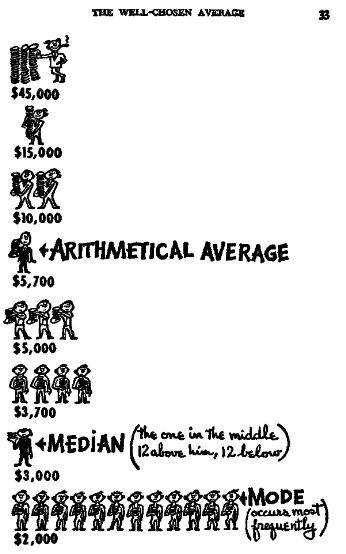
\includegraphics[width=0.4\textwidth]{wellchosenaverage}\\
  \vspace{5px}
  \small{From \emph{How to lie with statistics}, by Darrell Huff (p.33).}
\end{center}

\begin{description}
  \item[Arithmetic mean] \hfill \\
    This is the `usual' average value; it tells us where the `centre of mass' of the data lies. However,
    it might not be typical of any actual data value; see the diagram above, or consider that the
    mean of $\{13,15,16,80\} $ is 31, but no actual data value is anywhere near 31.
  \item[Median and quartiles] \hfill \\
    If we list out all the data values for our measurement in order and then pick the three quartiles (the \emph{lower quartile}
    is the value that 25\% of the values lie below, the \emph{median} is the value that 50\% of the values lie below, and the
    \emph{upper quartile} is the value that 75\% of values lie below), then we have some information about the `shape' of the
    data. If we have two populations to compare (female versus non-female.)
  \item[Mode] \hfill \\
    The \emph{mode} is the most common value for the measurement.
\end{description}

We also have measures of spread, which tell us how likely we are to find points far away from our central point.
\begin{description}
  \item[Range and inter-quartile range] \hfill \\
    These values, the difference between the maximum and minimum and between the two quartiles respectively, give us
    a rough idea of how spread out our data values are. However, they don't tell us whether the `typical' data value
    is close to or far away from the centre --- only how far apart the furthest data points are.
  \item[Variance and standard deviation] \hfill \\
    The \emph{variance} $ s^2 $ of a set of data is the mean of the squares of the distances of each point to the mean.
    \begin{displaymath}
      s^2 = \frac{\sum (x - \bar x)^2}{n}.
    \end{displaymath}
    The \emph{standard deviation} of the set is $ s $, the square root of the variance.
\end{description}

We will use the central points and the spread measurements of our sample to estimate the same values
for the population as a whole.

\subsection*{Drawing an inference}
We then need to take our \emph{statistics} and work out how sure we can be about the
\emph{parameters} of the population.

At this level, we won't go into the details too far. What we will do is assume that our
median value for our sample is a reasonable guess for the median value of our population,
and then write down an \emph{informal confidence interval}:
\begin{displaymath}
  \text{sample median} \pm 1.5 \cdot \frac{\text{IQR}}{\sqrt{n}}
\end{displaymath}
(where IQR is the inter-quartile range of the sample). Note: bigger sample size,
smaller informal confidence interval. (Why?)

The population median will lie within this range with 90\% confidence: if
we sample ten times, calculating this value each time, then on average nine of
these intervals will contain the population median.\footnote{Next year, we will
learn how to make this idea more useful by re-sampling the population a bunch of
times to make the confidence intervals we obtain smaller.}

In order to compare two subsets of a population, it is useful to use side-by-side
box and whisker graphs to visualise the shapes of the data sets. For example:
\begin{center}
  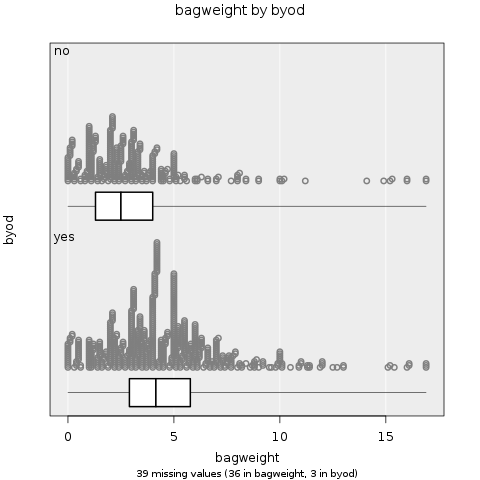
\includegraphics[width=0.5\textwidth]{stats-byod}
\end{center}


\clearpage
\subsection*{Questions}
\begin{questions}
  \question Consider a data set with at least three values. Suppose we increase the highest
            value by 10, and decrease the lowest by 5. Do the mean or the median change? Is
            it possible for the mode to change?
  \question Repeat (1), but now decrease the lowest value by 10 rather than 5 (so the increase
            of the highest value is the same as the decrease of the lowest).
  \question If a data set has an even number of points, is the median ever equal to a value in the set?
  \question Consider the numbers $ \{ 2, 3, 5, 5, 5, 7, 9 \} $. Which measure(s) of central tendancy (mean,
            median, or mode) makes sense in the following situations:
    \begin{parts}
      \item If the numbers represent colours of T-shirts ordered from a website?
      \item If the numbers represent distances from a point to given destinations?
      \item If the numbers are survey responses on a scale of 1--10?
    \end{parts}
  \question A set of five data values has a mean of 39. A new data point with value 17 is added to the set; what is the new mean?
  \question Compare and contrast the inter-quartile range and the standard deviation as measures of spread. Discuss the following
            statement: ``mean is to median as standard deviation is to range''.
  \question One important use of the standard deviation is Chebyshev's theorem: for any set of data, and for any constant $ k > 1 $, the
            proportion of the data that lies within $ k $ standard deviations on either side of the mean is at least $ 1 - 1/k^2 $.
    \begin{parts}
      \item If a set of data has mean $ \mu $ and standard deviation $ \sigma $, at least what proportion of the data lies within
            the range from $ \mu - 3\sigma $ to $ \mu + 3\sigma $?
      \item Show that if a set of data has mean $ \mu $ and standard deviation $ \sigma $, then (i) at least 75\% of the
            data lies in the range from $ \mu - 2\sigma $ to $ \mu + 2\sigma $; (ii) at least 93.8\% of the data lies in the
            range from $ \mu - 4\sigma $ to $ \mu + 4\sigma $.
    \end{parts}
  \question Consider the following data from the 2017 Census at School. (The question answered was `How much water did you drink yesterday?'.) Is
            there any significant difference between the Auckland and Wellington medians?
\begin{verbatim}
======================================================================================
                               iNZight Summary
--------------------------------------------------------------------------------------
        Primary variable of interest: region (categorical)
                  Secondary variable: drinkwater (numeric)

        Total number of observations: 1000
   Number omitted due to missingness: 68 (68 in drinkwater)
   Total number of observations used: 932
======================================================================================

Summary of drinkwater by region:
--------------------------------

                       Min   25%   Median    75%    Max    Mean      SD   Sample Size
     Auckland Region     0   250      700   1000   4000   799.1   724.7           471
   Wellington Region     0   250      600   1000   4000   774.6   702.1           461


======================================================================================
\end{verbatim}

  \question The following table shows the data collected from a sample of 1000 Census at School respondents (2017 survey),
            answering the question `In how many languages can you hold a conversation about a lot of every day things?'.
            The notation $ [a,b) $ means `all the numbers between $ a $ and $ b $, including $ a $ but not including $ b $'.
            \begin{center}
              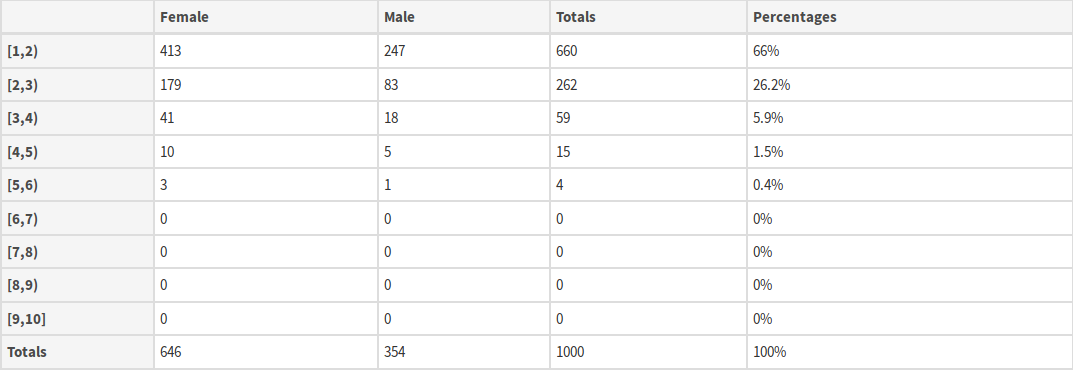
\includegraphics[width=\textwidth]{stats-languages}
            \end{center}
    \begin{parts}
      \item Calculate the statistics for the total sample. Hence write down a guess for the population
            measurement, and a confidence interval for that guess. Is it more or less than you would expect?
      \item Calculate the statistics for male and female respondents from the sample separately. Is there
            a significant difference between your sample medians? Consider the male and female populations
            of respondents. Can you conclude that, in general, one gender tends to be comfortable with
            more languages than the other? (Two populations are likely to have different population medians
            if the informal confidence intervals for the median of each don't overlap.)
    \end{parts}
  \question The following tables show the data collected from a sample of 1000 Census at School respondents answering the question `What
            is the main way you usually get to school?'. The first table is sampled from the 2009 data set, and the second from the 2017
            data set. Pick a mode of transport, make a hypothesis (with reasoning) as to whether there is likely to be any significant
            change in usage of your chosen mode over the eight years between the two surveys, and test your hypothesis.
            \begin{center}
              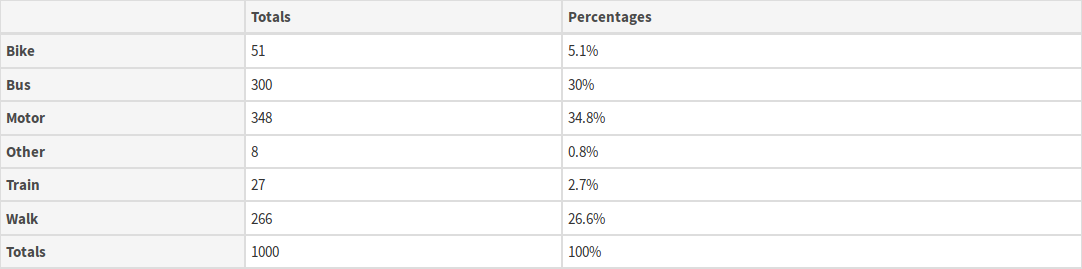
\includegraphics[width=\textwidth]{stats-transport2009}
            \end{center}
            \begin{center}
              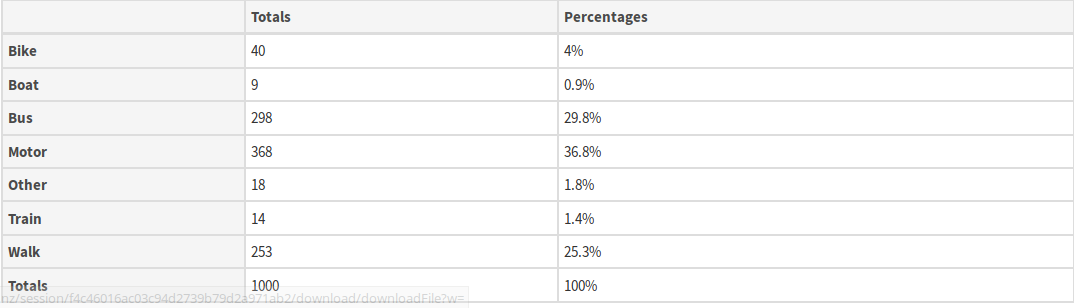
\includegraphics[width=\textwidth]{stats-transport2017}
            \end{center}
\end{questions}

\end{document}

